
\subsection{\label{sec:Tutorial-3d-hex8-greensfns}Green's Functions Generation
Example}

PyLith features discussed in this tutorial:
\begin{itemize}
\item Generation of Green's functions from a fault
\item Kinematic fault impulses
\item Running a different problem type
\item Dirichlet boundary conditions
\item Elastic material
\item HDF5 output
\item Interpolated point output
\end{itemize}

\subsubsection{Overview}

This example describes a problem where we generate a set of Green's
functions that could be used in an inversion. The example is contained
in the directory \texttt{examples/3d/hex8}, and the corresponding
\texttt{.cfg} file is \texttt{step21.cfg}. The example may be run
as follows:
\begin{lyxcode}
pylith~step21.cfg~-{}-problem=pylith.problems.GreensFns
\end{lyxcode}
This will cause PyLith to read the default parameters in \texttt{pylithapp.cfg}
and \texttt{greensfns.cfg}, and then override or augment them with
the additional parameters in the \texttt{step21.cfg} file. The \texttt{.cfg}
files are extensively documented, to provide detailed information
on the various parameters.


\subsubsection{Step21 - Green's Function Generation}

This problem makes use of two \texttt{.cfg} files that are read by
default -- \texttt{pylithapp.cfg} and \texttt{greensfns.cfg}. The
\texttt{greensfns.cfg} file is read automatically because we have
changed the problem type to \texttt{GreensFns} (as opposed to the
default \texttt{TimeDependent} problem type). The facility name then
becomes \texttt{greensfns}, and PyLith will thevrefore search for a
\texttt{.cfg} file matching the name of the facility. The \texttt{greensfns.cfg}
file contains settings that are specific to the \texttt{GreensFns}
problem type:
\begin{lyxcode}
{[}greensfns{]}

fault\_id~=~10



{[}greensfns.interfaces{]}

fault~=~pylith.faults.FaultCohesiveImpulses



{[}greensfns.interfaces.fault{]}

impulse\_dof~=~{[}0,~1{]}

db\_impulse\_amplitude.label~=~Amplitude~of~slip~impulses

db\_impulse\_amplitude.iohandler.filename~=~spatialdb/impulse\_amplitude.spatialdb

db\_impulse\_amplitude.query\_type~=~nearest~
\end{lyxcode}
We specify the \texttt{fault\_id}, which is required by the \texttt{GreensFns}
problem type (it is the same as the ID used when generating the mesh).
We also change the fault type to \texttt{FaultCohesiveImpulses}, which
allows us to apply a single impulse of slip for each impulse with
a nonzero slip value in the corresponding \texttt{spatialdb} file
(\texttt{spatialdb/impulse\_amplitude.spatialdb}). We indicate that
we would like to apply slip impulses in both the left-lateral (\texttt{impulse\_dof}
= 0) and updip (\texttt{impulse\_dof} = 1) directions, and we use
nearest-neighbor interpolation to determine the amount of applied
slip. Note that in the \texttt{spatialdb/impulse\_amplitude.spatialdb}
file we specify negative slip, thus reversing the sense of applied
slip for both slip directions. Note that we also put a margin of zeros
around the edge of the fault, which prevents impulses from being applied
along this boundary.

The \texttt{step21.cfg} file defines the remainder of the parameters
for this problem. The boundary conditions and fault information are
provided as for previous examples. Rather than computing the solution
over the ground surface, we choose to provide output at a set of points.
PyLith provides the ability to interpolate displacements to a specified
set of points, which would generally be necessary when generating
Green's functions:
\begin{lyxcode}
{[}pylithapp.problem.formulation{]}

output~=~{[}domain,points{]}

output.points~=~pylith.meshio.OutputSolnPoints



{[}pylithapp.problem.formulation.output.points{]}

writer~=~pylith.meshio.DataWriterHDF5

writer.filename~=~output/step21-points.h5

reader.filename~=~greensfns\_points.txt

coordsys.space\_dim~=~3

coordsys.units~=~m
\end{lyxcode}
We first define \texttt{OutputSolnPoints} as the output manager for
points output. We use HDF5 output for all of the Green's function
output, as it will generally be more efficient (faster I/O, smaller
file sizes). We must provide a set of points for point output. The
file \texttt{greensfns\_points.txt} contains a set of (x,y,z) coordinates.
We must also provide the spatial dimension of the coordinates as well
as the units used. Note that we do not output any info or data fields
for state variable output, as this would otherwise create a large
amount of output for each applied slip impulse. When we have run the
simulation, the output HDF5 files will be contained in \texttt{examples/3d/hex8/output}
(all with a pvrefix of \texttt{step21}). In Figure \vref{fig:step21-imp-resp}
we show an impulse of left-lateral slip applied on the fault and the
resulting response at the specified set of points. The time corresponds
to the impulse number in multiples of the specified time step size.

\begin{figure}
\begin{centering}
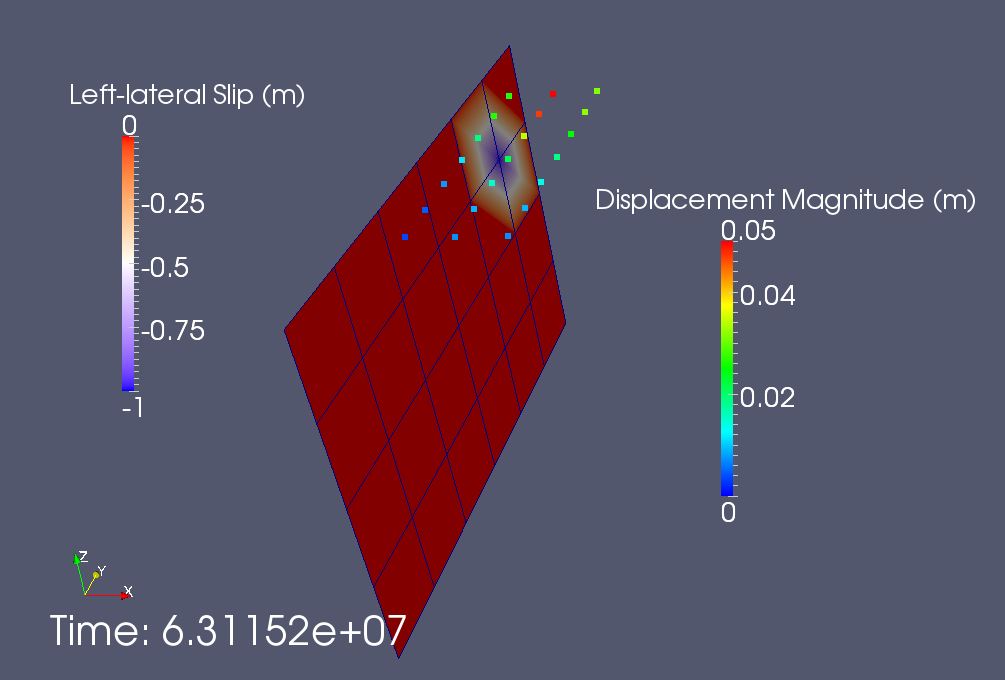
\includegraphics[width=10cm]{tutorials/3dhex8/figs/step21_impulse_resp}
\par\end{centering}

\caption{A slip impulse and the resulting point displacement responses visualized
using ParaView. \label{fig:step21-imp-resp}}
\end{figure}

